% Important: If latex complains about unicode characters,
% please use "\usepackage[utf8x]{inputenc}" in your preamble
% You can change the size of the picture by putting it into the construct:
% 1) \resizebox{10cm}{!}{"below picture"} to scale horizontally to 10 cm
% 2) \resizebox{!}{15cm}{"below picture"} to scale vertically to 15 cm
% 3) \resizebox{10cm}{15cm}{"below picture"} a combination of above two
% It is not recomended to use the scale option of the tikzpicture environment.
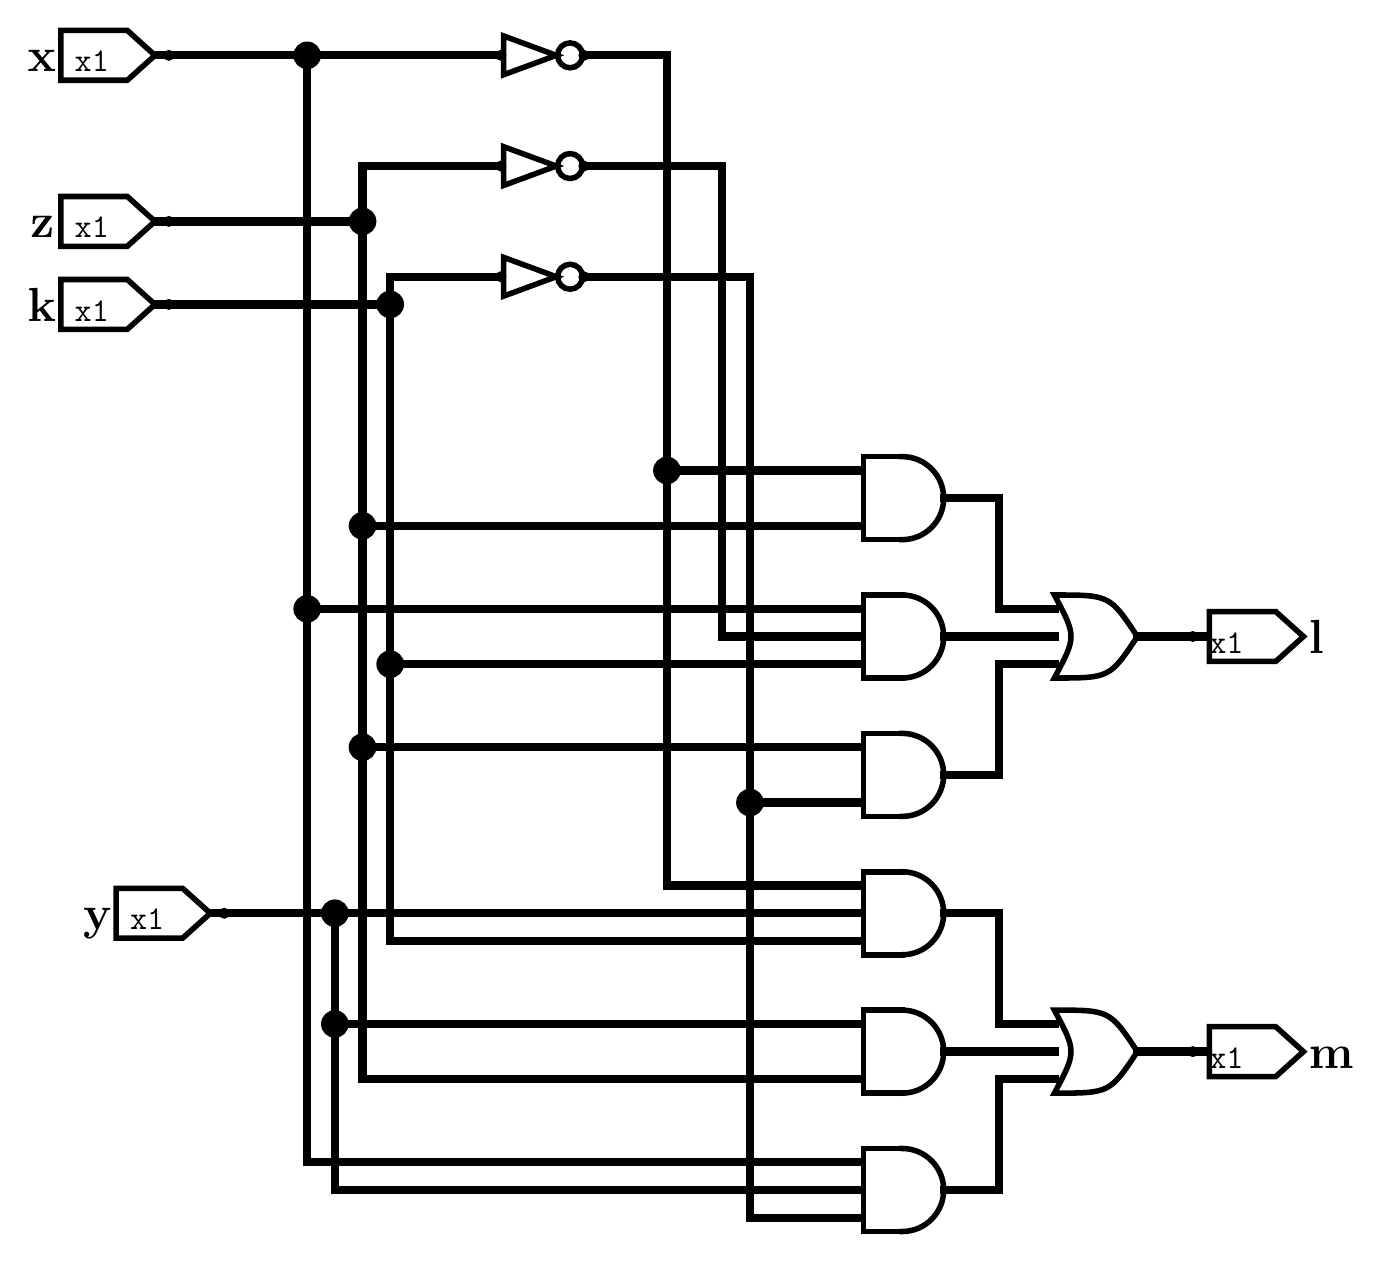
\begin{tikzpicture}[x=1pt,y=-1pt,line cap=rect]
\def\logisimfontA#1{\fontfamily{cmr}{#1}} % Replaced by logisim, original font was "SansSerif"
\def\logisimfontB#1{\fontfamily{cmtt}{#1}} % Replaced by logisim, original font was "Monospaced"
\definecolor{custcol_0_0_0}{RGB}{0, 0, 0}
\definecolor{custcol_ff_ff_ff}{RGB}{255, 255, 255}
\draw [line width=3.0pt, custcol_0_0_0 ]  (406.0,375.0) -- (426.0,375.0) ;
\draw [line width=3.0pt, custcol_0_0_0 ]  (106.0,15.0) -- (176.0,15.0) ;
\draw [line width=3.0pt, custcol_0_0_0 ]  (206.0,55.0) -- (256.0,55.0) -- (256.0,225.0) -- (306.0,225.0) ;
\draw [line width=3.0pt, custcol_0_0_0 ]  (126.0,185.0) -- (126.0,265.0) -- (306.0,265.0) ;
\draw [line width=3.0pt, custcol_0_0_0 ]  (176.0,55.0) -- (126.0,55.0) -- (126.0,75.0) -- (126.0,185.0) -- (306.0,185.0) ;
\draw [line width=3.0pt, custcol_0_0_0 ]  (306.0,235.0) -- (136.0,235.0) -- (136.0,105.0) -- (136.0,95.0) -- (176.0,95.0) ;
\draw [line width=3.0pt, custcol_0_0_0 ]  (306.0,435.0) -- (266.0,435.0) -- (266.0,285.0) -- (306.0,285.0) ;
\draw [line width=3.0pt, custcol_0_0_0 ]  (206.0,15.0) -- (236.0,15.0) -- (236.0,165.0) -- (306.0,165.0) ;
\draw [line width=3.0pt, custcol_0_0_0 ]  (136.0,235.0) -- (136.0,335.0) -- (306.0,335.0) ;
\draw [line width=3.0pt, custcol_0_0_0 ]  (116.0,325.0) -- (116.0,365.0) -- (306.0,365.0) ;
\draw [line width=3.0pt, custcol_0_0_0 ]  (406.0,225.0) -- (426.0,225.0) ;
\draw [line width=3.0pt, custcol_0_0_0 ]  (106.0,215.0) -- (306.0,215.0) ;
\draw [line width=3.0pt, custcol_0_0_0 ]  (236.0,165.0) -- (236.0,315.0) -- (306.0,315.0) ;
\draw [line width=3.0pt, custcol_0_0_0 ]  (206.0,95.0) -- (266.0,95.0) -- (266.0,285.0) ;
\draw [line width=3.0pt, custcol_0_0_0 ]  (126.0,265.0) -- (126.0,385.0) -- (306.0,385.0) ;
\draw [line width=3.0pt, custcol_0_0_0 ]  (116.0,365.0) -- (116.0,425.0) -- (306.0,425.0) ;
\fill [line width=3.0pt, custcol_0_0_0]  (136.0,105.0) ellipse (5.0 and 5.0 );
\fill [line width=3.0pt, custcol_0_0_0]  (136.0,235.0) ellipse (5.0 and 5.0 );
\fill [line width=3.0pt, custcol_0_0_0]  (106.0,15.0) ellipse (5.0 and 5.0 );
\fill [line width=3.0pt, custcol_0_0_0]  (116.0,365.0) ellipse (5.0 and 5.0 );
\fill [line width=3.0pt, custcol_0_0_0]  (126.0,185.0) ellipse (5.0 and 5.0 );
\fill [line width=3.0pt, custcol_0_0_0]  (126.0,75.0) ellipse (5.0 and 5.0 );
\fill [line width=3.0pt, custcol_0_0_0]  (106.0,215.0) ellipse (5.0 and 5.0 );
\fill [line width=3.0pt, custcol_0_0_0]  (236.0,165.0) ellipse (5.0 and 5.0 );
\fill [line width=3.0pt, custcol_0_0_0]  (126.0,265.0) ellipse (5.0 and 5.0 );
\fill [line width=3.0pt, custcol_0_0_0]  (116.0,325.0) ellipse (5.0 and 5.0 );
\fill [line width=3.0pt, custcol_0_0_0]  (266.0,285.0) ellipse (5.0 and 5.0 );
\draw [line width=2.0pt, custcol_0_0_0] (321.0,340.0) arc (90.0:-90.0:15.0 and 15.0 );
\draw [line width=2.0pt, custcol_0_0_0 ]  (321.0,310.0) -- (307.0,310.0) -- (307.0,340.0) -- (321.0,340.0) ;
\draw [line width=2.0pt, custcol_0_0_0] (321.0,290.0) arc (90.0:-90.0:15.0 and 15.0 );
\draw [line width=2.0pt, custcol_0_0_0 ]  (321.0,260.0) -- (307.0,260.0) -- (307.0,290.0) -- (321.0,290.0) ;
\draw [line width=2.0pt, custcol_0_0_0] (321.0,190.0) arc (90.0:-90.0:15.0 and 15.0 );
\draw [line width=2.0pt, custcol_0_0_0 ]  (321.0,160.0) -- (307.0,160.0) -- (307.0,190.0) -- (321.0,190.0) ;
\draw [line width=2.0pt, custcol_0_0_0] (321.0,390.0) arc (90.0:-90.0:15.0 and 15.0 );
\draw [line width=2.0pt, custcol_0_0_0 ]  (321.0,360.0) -- (307.0,360.0) -- (307.0,390.0) -- (321.0,390.0) ;
\draw [line width=3.0pt, custcol_0_0_0 ]  (336.0,325.0) -- (356.0,325.0) -- (356.0,365.0) -- (376.0,365.0) -- (376.0,365.0) ;
\draw [line width=3.0pt, custcol_0_0_0 ]  (336.0,375.0) -- (376.0,375.0) -- (376.0,375.0) ;
\draw [line width=3.0pt, custcol_0_0_0 ]  (376.0,385.0) -- (376.0,385.0) -- (356.0,385.0) -- (356.0,425.0) -- (336.0,425.0) ;
\draw [line width=2.0pt, custcol_0_0_0 ]  (406.0,375.0) .. controls  (396.0,360.0)  ..  (376.0,360.0) .. controls  (384.0,375.0)  ..  (376.0,390.0) .. controls  (396.0,390.0)  ..  (406.0,375.0) -- cycle ;
\draw [line width=2.0pt, custcol_0_0_0 ]  (196.0,55.0) -- (177.0,48.0) -- (177.0,62.0) -- cycle;
\draw [line width=2.0pt, custcol_0_0_0]  (201.0,55.0) ellipse (4.5 and 4.5 );
\fill [line width=2.0pt, custcol_0_0_0]  (206.0,55.0) ellipse (2.0 and 2.0 );
\fill [line width=2.0pt, custcol_0_0_0]  (176.0,55.0) ellipse (2.0 and 2.0 );
\draw [line width=3.0pt, custcol_0_0_0 ]  (336.0,175.0) -- (356.0,175.0) -- (356.0,215.0) -- (376.0,215.0) -- (376.0,215.0) ;
\draw [line width=3.0pt, custcol_0_0_0 ]  (336.0,225.0) -- (376.0,225.0) -- (376.0,225.0) ;
\draw [line width=3.0pt, custcol_0_0_0 ]  (336.0,275.0) -- (356.0,275.0) -- (356.0,235.0) -- (376.0,235.0) -- (376.0,235.0) ;
\draw [line width=2.0pt, custcol_0_0_0 ]  (406.0,225.0) .. controls  (396.0,210.0)  ..  (376.0,210.0) .. controls  (384.0,225.0)  ..  (376.0,240.0) .. controls  (396.0,240.0)  ..  (406.0,225.0) -- cycle ;
\draw [line width=2.0pt, custcol_0_0_0] (321.0,440.0) arc (90.0:-90.0:15.0 and 15.0 );
\draw [line width=2.0pt, custcol_0_0_0 ]  (321.0,410.0) -- (307.0,410.0) -- (307.0,440.0) -- (321.0,440.0) ;
\draw [line width=2.0pt, custcol_0_0_0 ]  (196.0,95.0) -- (177.0,88.0) -- (177.0,102.0) -- cycle;
\draw [line width=2.0pt, custcol_0_0_0]  (201.0,95.0) ellipse (4.5 and 4.5 );
\fill [line width=2.0pt, custcol_0_0_0]  (206.0,95.0) ellipse (2.0 and 2.0 );
\fill [line width=2.0pt, custcol_0_0_0]  (176.0,95.0) ellipse (2.0 and 2.0 );
\draw [line width=2.0pt, custcol_0_0_0] (321.0,240.0) arc (90.0:-90.0:15.0 and 15.0 );
\draw [line width=2.0pt, custcol_0_0_0 ]  (321.0,210.0) -- (307.0,210.0) -- (307.0,240.0) -- (321.0,240.0) ;
\draw [line width=2.0pt, custcol_0_0_0 ]  (196.0,15.0) -- (177.0,8.0) -- (177.0,22.0) -- cycle;
\draw [line width=2.0pt, custcol_0_0_0]  (201.0,15.0) ellipse (4.5 and 4.5 );
\fill [line width=2.0pt, custcol_0_0_0]  (206.0,15.0) ellipse (2.0 and 2.0 );
\fill [line width=2.0pt, custcol_0_0_0]  (176.0,15.0) ellipse (2.0 and 2.0 );
\draw [line width=3.0pt, custcol_0_0_0 ]  (430.0,375.0) -- (427.0,375.0) ;
\draw [line width=2.0pt, custcol_0_0_0 ]  (456.0,366.0) -- (466.0,375.0) -- (456.0,384.0) -- (432.0,384.0) -- (432.0,366.0) -- cycle;
\logisimfontB{\fontsize{12pt}{12pt}\selectfont\node[inner sep=0, outer sep=0, custcol_0_0_0, anchor=base west] at  (432.0,381.0)  {x1};}
\logisimfontA{\fontsize{16pt}{16pt}\fontseries{bx}\selectfont\node[inner sep=0, outer sep=0, custcol_0_0_0, anchor=base west] at  (468.0,381.0)  {m};}
\fill [line width=2.0pt, custcol_0_0_0]  (426.0,375.0) ellipse (2.0 and 2.0 );
\draw [line width=3.0pt, custcol_0_0_0 ]  (430.0,225.0) -- (427.0,225.0) ;
\draw [line width=2.0pt, custcol_0_0_0 ]  (456.0,216.0) -- (466.0,225.0) -- (456.0,234.0) -- (432.0,234.0) -- (432.0,216.0) -- cycle;
\logisimfontB{\fontsize{12pt}{12pt}\selectfont\node[inner sep=0, outer sep=0, custcol_0_0_0, anchor=base west] at  (432.0,231.0)  {x1};}
\logisimfontA{\fontsize{16pt}{16pt}\fontseries{bx}\selectfont\node[inner sep=0, outer sep=0, custcol_0_0_0, anchor=base west] at  (468.0,231.0)  {l};}
\fill [line width=2.0pt, custcol_0_0_0]  (426.0,225.0) ellipse (2.0 and 2.0 );
\draw [line width=3.0pt, custcol_0_0_0 ]  (71.0,325.0) -- (76.0,325.0) -- (116.0,325.0) -- (306.0,325.0) ;
\draw [line width=2.0pt, custcol_0_0_0 ]  (61.0,334.0) -- (71.0,325.0) -- (61.0,316.0) -- (37.0,316.0) -- (37.0,334.0) -- cycle;
\logisimfontB{\fontsize{12pt}{12pt}\selectfont\node[inner sep=0, outer sep=0, custcol_0_0_0, anchor=base west] at  (42.0,331.0)  {x1};}
\logisimfontA{\fontsize{16pt}{16pt}\fontseries{bx}\selectfont\node[inner sep=0, outer sep=0, custcol_0_0_0, anchor=base west] at  (25.0,331.0)  {y};}
\fill [line width=2.0pt, custcol_0_0_0]  (76.0,325.0) ellipse (2.0 and 2.0 );
\draw [line width=3.0pt, custcol_0_0_0 ]  (51.0,15.0) -- (56.0,15.0) -- (106.0,15.0) -- (106.0,215.0) -- (106.0,415.0) -- (306.0,415.0) ;
\draw [line width=2.0pt, custcol_0_0_0 ]  (41.0,24.0) -- (51.0,15.0) -- (41.0,6.0) -- (17.0,6.0) -- (17.0,24.0) -- cycle;
\logisimfontB{\fontsize{12pt}{12pt}\selectfont\node[inner sep=0, outer sep=0, custcol_0_0_0, anchor=base west] at  (22.0,21.0)  {x1};}
\logisimfontA{\fontsize{16pt}{16pt}\fontseries{bx}\selectfont\node[inner sep=0, outer sep=0, custcol_0_0_0, anchor=base west] at  (5.0,21.0)  {x};}
\fill [line width=2.0pt, custcol_0_0_0]  (56.0,15.0) ellipse (2.0 and 2.0 );
\draw [line width=3.0pt, custcol_0_0_0 ]  (51.0,75.0) -- (56.0,75.0) -- (126.0,75.0) ;
\draw [line width=2.0pt, custcol_0_0_0 ]  (41.0,84.0) -- (51.0,75.0) -- (41.0,66.0) -- (17.0,66.0) -- (17.0,84.0) -- cycle;
\logisimfontB{\fontsize{12pt}{12pt}\selectfont\node[inner sep=0, outer sep=0, custcol_0_0_0, anchor=base west] at  (22.0,81.0)  {x1};}
\logisimfontA{\fontsize{16pt}{16pt}\fontseries{bx}\selectfont\node[inner sep=0, outer sep=0, custcol_0_0_0, anchor=base west] at  (6.0,81.0)  {z};}
\fill [line width=2.0pt, custcol_0_0_0]  (56.0,75.0) ellipse (2.0 and 2.0 );
\draw [line width=3.0pt, custcol_0_0_0 ]  (51.0,105.0) -- (56.0,105.0) -- (136.0,105.0) ;
\draw [line width=2.0pt, custcol_0_0_0 ]  (41.0,114.0) -- (51.0,105.0) -- (41.0,96.0) -- (17.0,96.0) -- (17.0,114.0) -- cycle;
\logisimfontB{\fontsize{12pt}{12pt}\selectfont\node[inner sep=0, outer sep=0, custcol_0_0_0, anchor=base west] at  (22.0,111.0)  {x1};}
\logisimfontA{\fontsize{16pt}{16pt}\fontseries{bx}\selectfont\node[inner sep=0, outer sep=0, custcol_0_0_0, anchor=base west] at  (5.0,111.0)  {k};}
\fill [line width=2.0pt, custcol_0_0_0]  (56.0,105.0) ellipse (2.0 and 2.0 );
\end{tikzpicture}

